%%%%%%%%%%%%%%%%%%%%%%%%%%%%%%%%%%%%%%%%%
% fphw Assignment
% LaTeX Template
% Version 1.0 (27/04/2019)
%
% This template originates from:
% https://www.LaTeXTemplates.com
%
% Authors:
% Class by Felipe Portales-Oliva (f.portales.oliva@gmail.com) with template 
% content and modifications by Vel (vel@LaTeXTemplates.com)
%
% Template (this file) License:
% CC BY-NC-SA 3.0 (http://creativecommons.org/licenses/by-nc-sa/3.0/)
%
%%%%%%%%%%%%%%%%%%%%%%%%%%%%%%%%%%%%%%%%%

%----------------------------------------------------------------------------------------
%	PACKAGES AND OTHER DOCUMENT CONFIGURATIONS
%----------------------------------------------------------------------------------------

\documentclass[
	12pt, % Default font size, values between 10pt-12pt are allowed
	%letterpaper, % Uncomment for US letter paper size
	%spanish, % Uncomment for Spanish
]{fphw}

% Template-specific packages
\usepackage[utf8]{inputenc} % Required for inputting international characters
\usepackage[T1]{fontenc} % Output font encoding for international characters
\usepackage{mathpazo} % Use the Palatino font

\usepackage{graphicx} % Required for including images

\usepackage{booktabs} % Required for better horizontal rules in tables

\usepackage{listings} % Required for insertion of code
\usepackage{longtable,booktabs}
\usepackage{enumerate} % To modify the enumerate environment
%codes setting
\RequirePackage{listings}
\RequirePackage{xcolor}
\definecolor{dkgreen}{rgb}{0,0.6,0}
\definecolor{gray}{rgb}{0.5,0.5,0.5}
\definecolor{mauve}{rgb}{0.58,0,0.82}
\lstset{
	numbers=left,  
	frame=tb,
	aboveskip=3mm,
	belowskip=3mm,
	showstringspaces=false,
	columns=flexible,
	framerule=1pt,
	rulecolor=\color{gray!35},
	backgroundcolor=\color{gray!5},
	basicstyle={\ttfamily},
	numberstyle=\tiny\color{gray},
	keywordstyle=\color{blue},
	commentstyle=\color{dkgreen},
	stringstyle=\color{mauve},
	breaklines=true,
	breakatwhitespace=true,
	tabsize=3,
}
%----------------------------------------------------------------------------------------
%	ASSIGNMENT INFORMATION
%----------------------------------------------------------------------------------------

\title{Homework \#3} % Assignment title

\author{Hang Chen} % Student name


\institute{Boise State University \\ Department of geoscience} % Institute or school name

\class{GEOS 422 / GEOPH 522: Data Analysis and Geostatistics} % Course or class name


%----------------------------------------------------------------------------------------

\begin{document}

\maketitle % Output the assignment title, created automatically using the information in the custom commands above

%----------------------------------------------------------------------------------------
%	ASSIGNMENT CONTENT
%----------------------------------------------------------------------------------------

\section*{Question 1}

\begin{problem}
Fit polynomial models of degree 0-4 to the velocity vs. depth data using MATLAB's polyfit.m function.
Evaluate the model at each measured depth using polyval.m. Plot the 5 model curves with the original
data, and state the root mean squared error in the legend:

	\begin{equation}
	R M S E=\sqrt{\frac{1}{N} \sum_{i=1}^{N}\left(v_{m}(z)-v_{o}(z)\right)^{2}}
	\end{equation}

\end{problem}




%------------------------------------------------

\subsection*{Answer}
The plot

\begin{figure}[htbp]
	\centering
	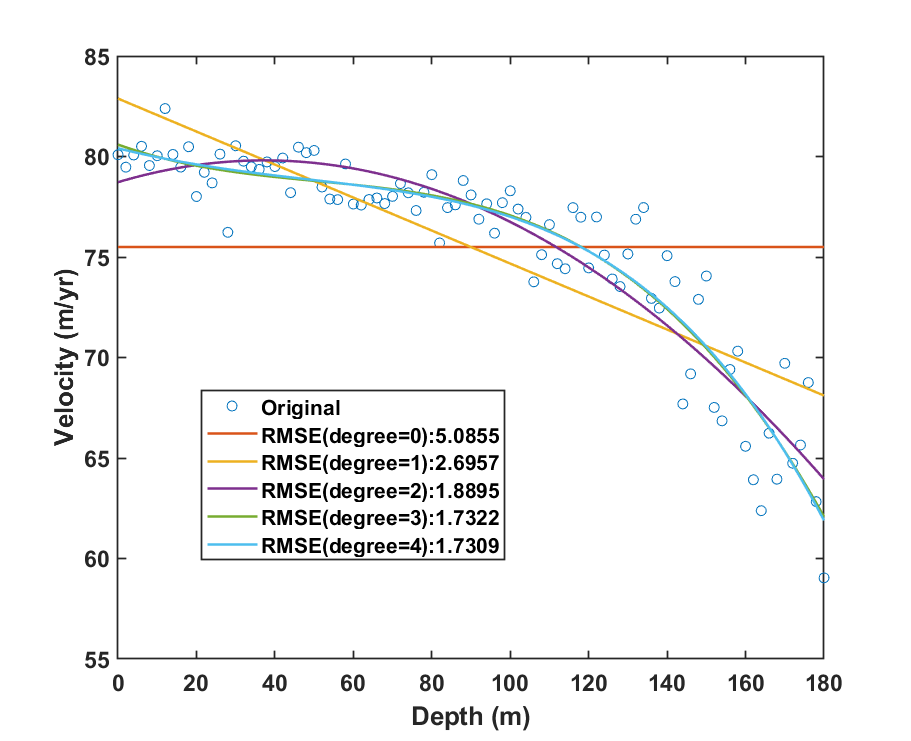
\includegraphics[width=0.8\columnwidth]{Q1.png} 
	\caption{Fit polynomial models of degree 0-4 to the velocity vs. depth data}
\end{figure}

The codes for fitting polynomial models of degree 0-4 to the velocity vs. depth data


\begin{lstlisting}[language=Matlab,escapeinside=``]
degree=0:4;%initial the degree
vtest=zeros(length(vel),length(degree));%initial the vtest
for i=1:length(degree)   
P=polyfit(depth,vel,degree(i));% fit a line to the data;
vtest(:,i)=polyval(P,depth);% evaluate at all depth
rmse(i)=sqrt(mean((vtest(:,i)-vel).^2));% calculate the rmse
end

%codes for plot
figure;
clf
plot(depth,vel,'o') %plot the original data
hold on
plot(depth,vtest(:,1),'linewidth',1.5) %plot the data from models of degree 0
hold on
plot(depth,vtest(:,2),'linewidth',1.5) %plot the data from models of degree 1
hold on
plot(depth,vtest(:,3),'linewidth',1.5) %plot the data from models of degree 2
hold on
plot(depth,vtest(:,4),'linewidth',1.5) %plot the data from models of degree 3
hold on
plot(depth,vtest(:,5),'linewidth',1.5) %plot the data from models of degree 4
legend('Original',['RMSE(degree=0):',num2str(rmse(1))]...
,['RMSE(degree=1):',num2str(rmse(2))]...
,['RMSE(degree=2):',num2str(rmse(3))]...
,['RMSE(degree=3):',num2str(rmse(4))]...
,['RMSE(degree=4):',num2str(rmse(5))])%set the legend

xlabel('Depth (m)')% for the label of x axis
ylabel('Velocity (m/yr)')% for the label of y axis
set(gca,'LineWidth',1,'FontSize',14,'FontWeight','bold')
print('Q1','-dpng')

\end{lstlisting}


%----------------------------------------------------------------------------------------

\section*{Question 2}

\begin{problem}
	We fit these 5 models using all of the data for parameter estimation, and therefore we don't have any
	information about the uncertainty in these parameter values, nor do we know the uncertainty in the RMSE
	for each model. To provide estimates of uncertainties in model parameters, repeat the above, but fit the
	models to a random sampling of 90\% of the original data. Store the parameters for each model, and repeat
	1000 times (Monte-Carlo). Report the model parameters in a table, using the mean and standard deviation
	of the 1000 parameter estimates.
	
\end{problem}

%------------------------------------------------

\subsection*{Answer}

The results are shown in the table below
\begin{longtable}[h]{@{}llll@{}}
	\toprule
	Degrees & Variables & Mean & Standard deviation\tabularnewline
	\midrule
	\endhead
	0 & A\textsubscript{0} & 75.4926 & 0.1776\tabularnewline
	& RMSE & 5.0829 & 0.1487\tabularnewline
	1 & A\textsubscript{0} & 80.2905 & 0.1713\tabularnewline
	& A\textsubscript{1} & -0.0821 & 0.0023\tabularnewline
	& RMSE & 2.6883 & 0.0826\tabularnewline
	2 & A\textsubscript{0} & 78.7126 & 0.1561\tabularnewline
	& A\textsubscript{1} & 0.0585 & 0.0048\tabularnewline
	& A\textsubscript{2} & -7.8134e-04 & 3.0373e-05\tabularnewline
	& RMSE & 1.8864 & 0.0550\tabularnewline
	3 & A\textsubscript{0} & 80.5932 & 0.1581\tabularnewline
	& A\textsubscript{1} & -0.0704 & 0.0098\tabularnewline
	& A\textsubscript{2} & 0.0010 & 1.5393e-04\tabularnewline
	& A\textsubscript{3} & -6.6583e-06 & 6.3588e-07\tabularnewline
	& RMSE & 1.7260 & 0.0574\tabularnewline
	4 & A\textsubscript{0} & 80.4129 & 0.1670\tabularnewline
	& A\textsubscript{1} & -0.0486 & 0.0177\tabularnewline
	& A\textsubscript{2} & 4.6153e-04 & 4.8591e-04\tabularnewline
	& A\textsubscript{3} & -1.8307e-06 & 4.6050e-06\tabularnewline
	& A\textsubscript{4} & -1.3398e-08 & 1.3892e-08\tabularnewline
	& RMSE & 1.7231 & 0.0595\tabularnewline
	\bottomrule
\end{longtable}


The results can be got by the codes:
\begin{lstlisting}[language=Matlab,escapeinside=``]
%I use the getTrain function in this question for convenience 
%The getTrain function is defind by class
degree=0:4;%initial the degree
pTrain=0.9;%define the pecent that's used in polynomial fit
nMC=1000; %times for Monte-Carlo
rmseCV=zeros(nMC,length(degree)); % initializing
for q=1:length(degree)
for p=1:nMC
[trainset, ~] = getTrainTest([depth vel],pTrain);%get 90% data
ztrain=trainset(:,1); % depths for training
vtrain=trainset(:,2); % velocity for training
PP{q}(p,:)=polyfit(ztrain,vtrain,degree(q));% fit a line to the data;
vm=polyval(PP{q}(p,:),ztrain); % evaluate at the train depths
rmseCV(p,q)=sqrt(mean((vtrain-vm).^2));% calculate the RMSE
end
end

%degree=0
mean_a0_0=mean(PP{1})%get the mean of A0 when degree=0
std_a0_0=std(PP{1})%get the standard deviation of A0 when degree=0
mean_rmse_0=mean(rmseCV(:,1))%get the mean of RMSE when degree=0
std_rmse_0=std(rmseCV(:,1))%get the standard deviation of RMSE when degree=0

%degree=1
mean_a1_1=mean(PP{2}(:,1))%get the mean of A1 when degree=1
std_a1_1=std(PP{2}(:,1))%get the standard deviation of A1 when degree=1
mean_a0_1=mean(PP{2}(:,2))%get the mean of A0 when degree=1
std_a0_1=std(PP{2}(:,2))%get the standard deviation of A0 when degree=1
mean_rmse_1=mean(rmseCV(:,2))%get the mean of RMSE when degree=1
std_rmse_1=std(rmseCV(:,2))%get the standard deviation of RMSE when degree=1

%degree=2
mean_a2_2=mean(PP{3}(:,1))%get the mean of A2 when degree=2
std_a2_2=std(PP{3}(:,1))%get the standard deviation of A2 when degree=2
mean_a1_2=mean(PP{3}(:,2))%get the mean of A1 when degree=2
std_a1_2=std(PP{3}(:,2))%get the standard deviation of A1 when degree=2
mean_a0_2=mean(PP{3}(:,3))%get the mean of A0 when degree=2
std_a0_2=std(PP{3}(:,3))%get the standard deviation of A0 when degree=2
mean_rmse_2=mean(rmseCV(:,3))%get the mean of RMSE when degree=2
std_rmse_2=std(rmseCV(:,3))%get the standard deviation of RMSE when degree=2

%degree=3
mean_a3_3=mean(PP{4}(:,1))%get the mean of A3 when degree=3
std_a3_3=std(PP{4}(:,1))%get the standard deviation of A3 when degree=3
mean_a2_3=mean(PP{4}(:,2))%get the mean of A2 when degree=3
std_a2_3=std(PP{4}(:,2))%get the standard deviation of A2 when degree=3
mean_a1_3=mean(PP{4}(:,3))%get the mean of A1 when degree=3
std_a1_3=std(PP{4}(:,3))%get the standard deviation of A1 when degree=3
mean_a0_3=mean(PP{4}(:,4))%get the mean of A0 when degree=3
std_a0_3=std(PP{4}(:,4))%get the standard deviation of A0 when degree=3
mean_rmse_3=mean(rmseCV(:,4))%get the mean of RMSE when degree=3
std_rmse_3=std(rmseCV(:,4))%get the standard deviation of RMSE when degree=3

%degree=4
mean_a4_4=mean(PP{5}(:,1))%get the mean of A3 when degree=4
std_a4_4=std(PP{5}(:,1))%get the standard deviation of A3 when degree=4
mean_a3_4=mean(PP{5}(:,2))%get the mean of A3 when degree=4
std_a3_4=std(PP{5}(:,2))%get the standard deviation of A3 when degree=4
mean_a2_4=mean(PP{5}(:,3))%get the mean of A2 when degree=4
std_a2_4=std(PP{5}(:,3))%get the standard deviation of A2 when degree=4
mean_a1_4=mean(PP{5}(:,4))%get the mean of A1 when degree=4
std_a1_4=std(PP{5}(:,4))%get the standard deviation of A1 when degree=4
mean_a0_4=mean(PP{5}(:,5))%get the mean of A0 when degree=4
std_a0_4=std(PP{5}(:,5))%get the standard deviation of A0 when degree=4
mean_rmse_4=mean(rmseCV(:,5))%get the mean of RMSE when degree=4
std_rmse_4=std(rmseCV(:,5))%get the standard deviation of RMSE when degree=4

\end{lstlisting}



%----------------------------------------------------------------------------------------

\section*{Question 3}

\begin{problem}
Perform a cross-validation, using 90\% of the data to fit the 5 polynomial models, and the remaining 10\% of
data to test, repeating 1000 times. Plot the distribution of RMSE values for each degree polynomial.
\end{problem}

%------------------------------------------------

\subsection*{Answer} 
 The distribution plot

\begin{figure}[htbp]
	\centering
	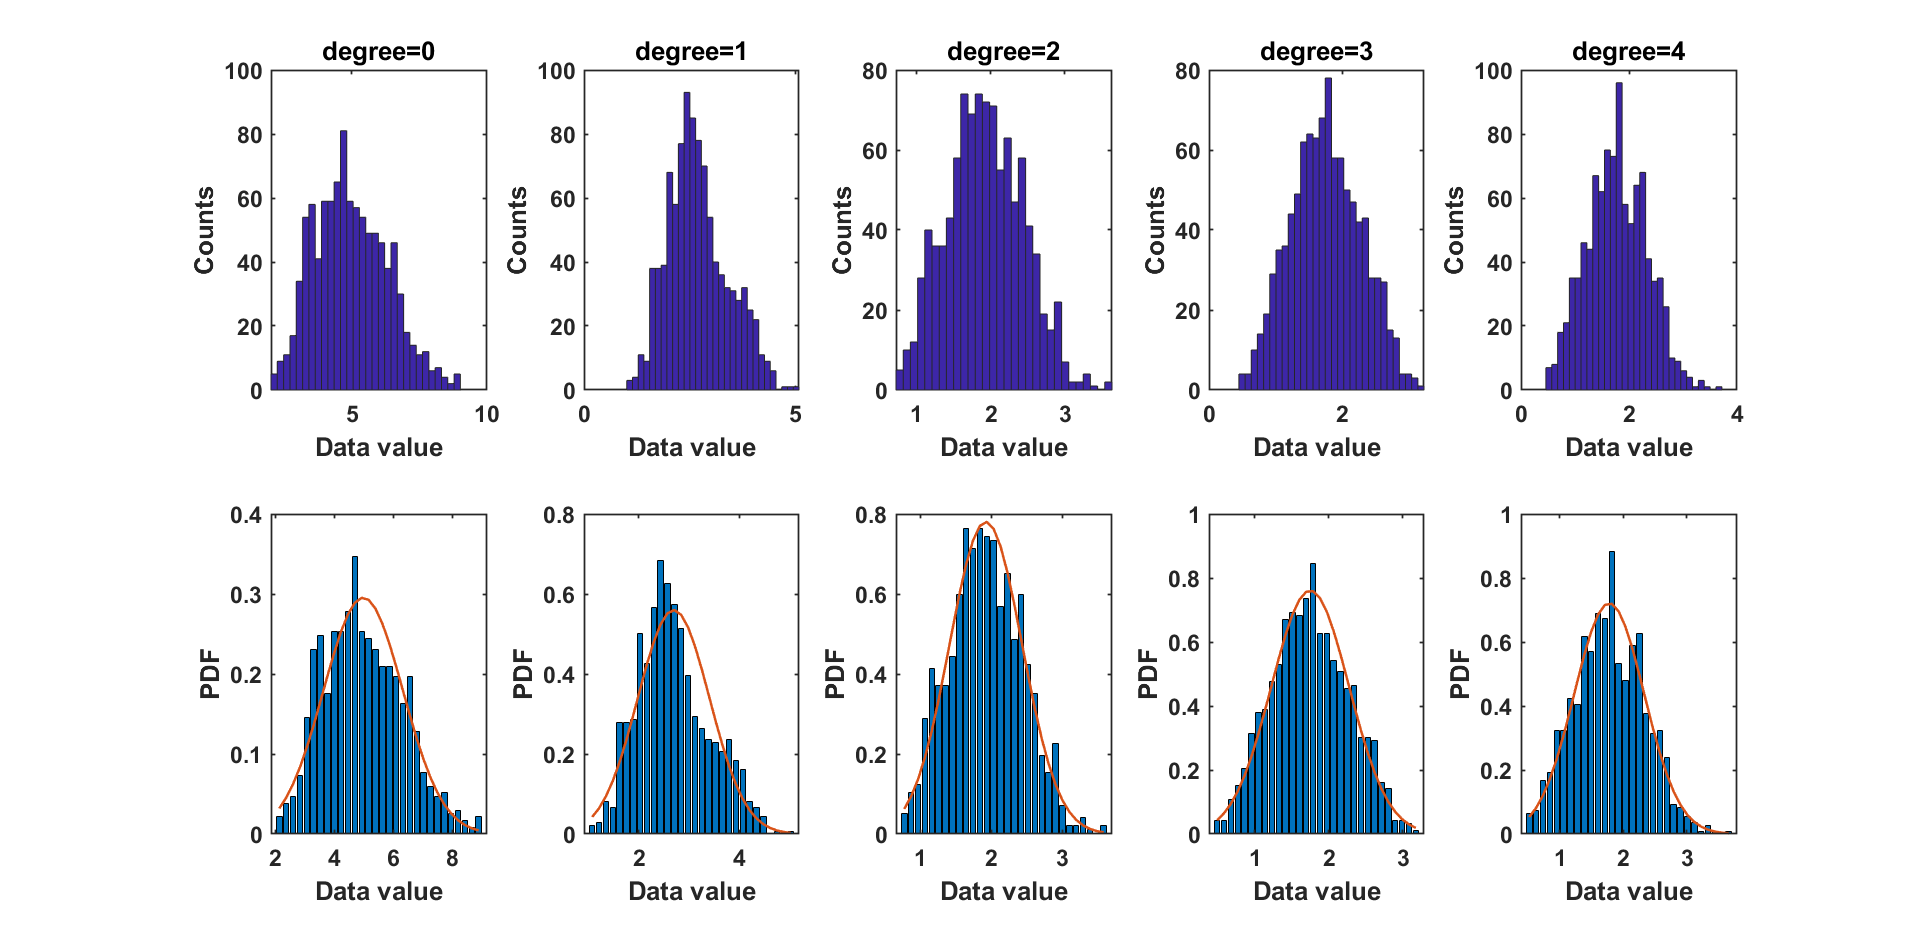
\includegraphics[width=1\columnwidth]{Q3.png} 
	\caption{The distribution of RMSE values for each degree polynomial(the above is histogram and the below is relative density histogram).}
\end{figure}

The codes for getting RMSE values for each degree polynonmial

\begin{lstlisting}[language=Matlab,escapeinside=``]
%I use the getTrain function in this question for convenience 
%The getTrain function is defind by class
%I also use the function defined plotRDH in HW2 to plot relative density hist

degree=0:4;%initial the degree
pTrain=0.9;%define the pecent that's used in polynomial fit
nMC=1000; %times for Monte-Carlo
rmseCV=zeros(nMC,length(degree)); % initializing
for q=1:length(degree)
for p=1:nMC
[trainset, testset] = getTrainTest([depth vel],pTrain);%get 90% data
ztrain=trainset(:,1); % depths for training
vtrain=trainset(:,2); % velocity for training
ztest=testset(:,1);% depths for test
vtest=testset(:,2);% velocity for test
PPP{q}(p,:)=polyfit(ztrain,vtrain,degree(q));% fit a line to the data;
vm=polyval(PPP{q}(p,:),ztest); % evaluate at the test depths
rmseCV(p,q)=sqrt(mean((vtest-vm).^2));% calculate the RMSE
end
end

bins=30;% set the bins
figure;

% plot the histgram 
for i=1:5
subplot(2,5,i)
hist(rmseCV(:,i),bins) %degree from 0 to 4
title(['degree=',num2str(i-1)])
xlabel('Data value')% for the label of x axis
ylabel('Counts')% for the label of y axis
set(gca,'LineWidth',1,'FontSize',14,'FontWeight','bold')
end
% plot the relative density histgram 
for i=1:5
subplot(2,5,i+5)
plotRDH(rmseCV(:,i),bins);%degree from 0 to 4
end
print('Q3','-dpng')
\end{lstlisting}




%----------------------------------------------------------------------------------------
\clearpage
\section*{Question 4 }

\begin{problem}
Use a moving window average to estimate the velocity as a function of depth, and plot with the data for a
window size of 3,10, and 50 meters.
\end{problem}

%------------------------------------------------

\subsection*{Answer}

The plot for using a moving window average to estimate the velocity as a function of depth,

\begin{figure}[htbp]
	\centering
	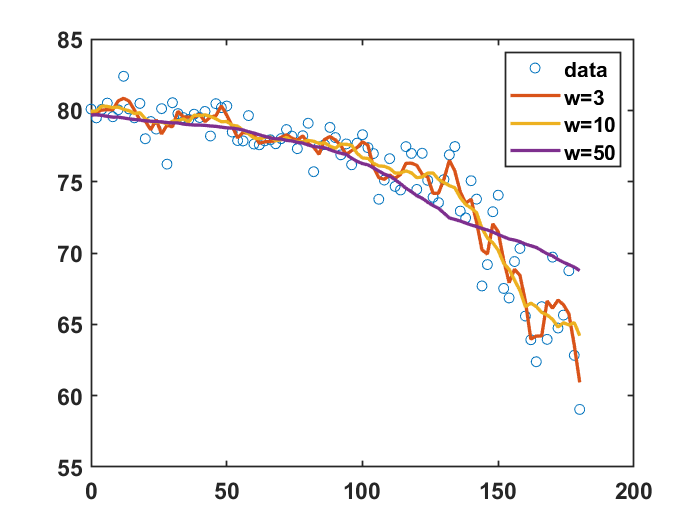
\includegraphics[width=0.8\columnwidth]{Q4.png} 
	\caption{Plot with the data for a
		window size of 3,10, and 50 meters with moving window average}
\end{figure}


The codes for  moving window average to estimate the velocity as a function of depth

\begin{lstlisting}[language=Matlab,escapeinside=``]

winsize=[3 10 50];% initial the windows' size
z0=0:2:180; %the points for the window average

for q=1:length(winsize)
for p=1:length(z0)
Ix=find(depth>(z0(p)-winsize(q)) & depth<(z0(p)+winsize(q))); % find values within window
um(p,q)=mean(vel(Ix)); % take mean within window
end
end
figure; 
plot(depth,vel,'o') %plot the original data
hold on
plot(z0,um,'linewidth',2) %plot the moving window average data
legend('data','w=3','w=10','w=50')
set(gca,'LineWidth',1,'FontSize',14,'FontWeight','bold')
print('Q4','-dpng')

\end{lstlisting}





%----------------------------------------------------------------------------------------

\section*{Question 5 }

\begin{problem}
Repeat, using a weighted moving window average (non-parametric smooth), for a window size of 3,10, and
50 meters.

\end{problem}

%------------------------------------------------

\subsection*{Answer}

The plot for using a weighted moving window average to estimate the velocity as a function of depth,

\begin{figure}[htbp]
	\centering
	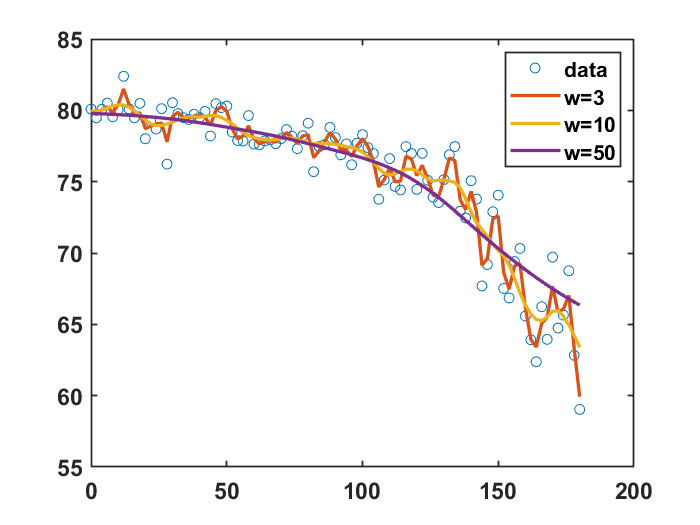
\includegraphics[width=0.8\columnwidth]{Q5.png} 
	\caption{Plot with the data for a
		window size of 3,10, and 50 meters with weighted moving window average}
\end{figure}

The codes for  a weighted moving window average (non-parametric smooth)

\begin{lstlisting}[language=Matlab,escapeinside=``]

% I use the function nanparametric_smooth defined in class

winsize=[3 10 50];% initial the windows' size
z0=0:2:180;%the points for the window average

for q=1:length(winsize)   
ymod(q,:) = nonparametric_smooth(depth,vel,z0,winsize(q));%using a weighted moving window average
end

figure; 
plot(depth,vel,'o') %plot the original data
hold on
plot(z0,ymod,'linewidth',2) %plot the moving window average data
legend('data','w=3','w=10','w=50')
set(gca,'LineWidth',1,'FontSize',14,'FontWeight','bold')
print('Q5','-dpng')
\end{lstlisting}

The nonparametric\_smooth function is defined

\begin{lstlisting}[language=Matlab,escapeinside=``]
function ymod = nonparametric_smooth(x,y,xmod,winsize)
% SNTX: ymod = nonparametric_smooth(x,y,xmod,winsize)
% this function smooths a 2-d dataset using a bisquare kernel
% INPUT: x = independent variable [n,1]
%        y = dependent variable [n,1]
%      xmod = locations of estimates [*,1]
%    winsize = size of the window (same units as x)
% OUTPUT ymod = nonparametric smoothed estimate
x=x(:); y=y(:); xmod=xmod(:);
ymod=zeros(size(xmod));
for i=1:length(xmod)
dist=sqrt((x-xmod(i)).^2); % distance from each data point to the estimate location
Ix=find(dist<winsize); % indicies to data within window
Ix=Ix(isfinite(y(Ix)));% removing NaNs
if isempty(Ix)
ymod(i)=NaN; % use Nan if no data within window
else
w=15/16*(1-(dist(Ix)/winsize).^2).^2; % bisquare kernel
ymod(i)=sum(w.*y(Ix))./sum(w); % unbiased estimate
end
end


\end{lstlisting}

\clearpage
\section*{Question 6 }

\begin{problem}
Find the optimum window size for the weighted moving window average model.
	
\end{problem}

\subsection*{Answer}


In this problem, I use 90\% of dataset to get the weighted moving window average model and 10\% of dataset for getting the RMSE. Because the data are randomly sampled from dataset, the results will change everytime I run the codes.

\textbf{Therefore, what I show here is just one of my tests, because of randomly sampling approach}. If you want to see more results, please run my codes. In this test, the best window size is 26 and the regarding RMSE is 0.6569.


\begin{figure}[htbp]
	\centering
	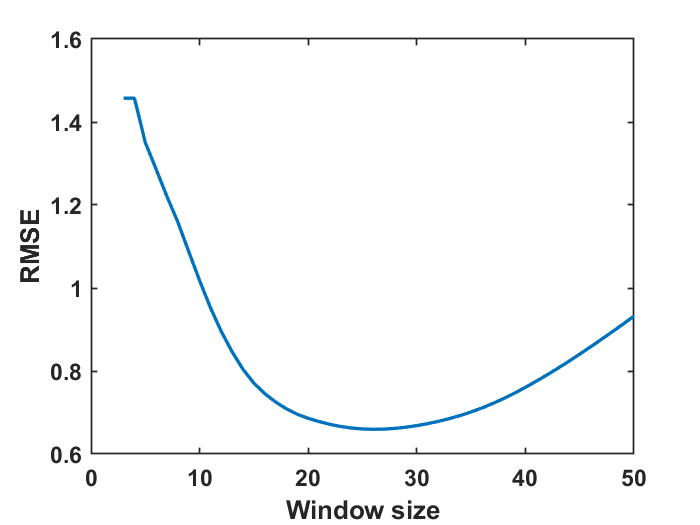
\includegraphics[width=0.6\columnwidth]{Q6_1.png} 
	\caption{RMSE versus windows length}
\end{figure}


\begin{lstlisting}[language=Matlab,escapeinside=``]
%first approach that I use the RMSE between the nonparametric models with
%physical models

pmodel=0.9;%define the pecent that's used in finding nonparametric models

g=9.8; % [m/s^2]
rho=917; % [kg/m^3]
theta=10*pi/180; % convert slope angle to rad
A=5e-18;%inital guess of A
n=3;%initial guess of n

um3=vel(1)-A.*(rho*g*sin(theta)).^n.*depth.^(n+1); % Eq 6 in HW3

winsize=[1:50];% initial the windows' size

[trainset, valiset] = getTrainTest([depth vel],pmodel);%get 90% data for model and 10% for validation

for q=1:length(winsize)


ymod1= nonparametric_smooth(trainset(:,1),trainset(:,2),valiset(:,1),winsize(q));%using a weighted moving window average
%, validation data for the location of esimation

RMSE(q)=sqrt(mean((ymod1-valiset(:,2)).^2));% calculate the RMSE
end

[va,minloc]=min(RMSE) %output the minimum RMSE and locaiton

figure
plot(winsize,RMSE,'linewidth',2)%plot the winsize versus the RMSE
xlabel('Window size')
ylabel('RMSE')
set(gca,'LineWidth',1,'FontSize',14,'FontWeight','bold')
print('Q6_1','-dpng')

\end{lstlisting} 



%----------------------------------------------------------------------------------------



\section*{Question 7 }

\begin{problem}
Using the measured velocity at a depth of z = 0 m for the surface velocity, $u_{x,surf}$, find the optimum values
for the 
ow law parameters A and n, using the grid search (brute-force) method. Note the MATLAB function
polyfit.m can't be used in this case.
	
\end{problem}


\subsection*{Answer}

The result from the brute-force method is that optimum A=9.0000e-18, n=2.9500 and the regarding RMSE=1.9523.


The codes for  grid search (brute-force) method to find optimal A and n
\begin{lstlisting}[language=Matlab,escapeinside=``]

% brute force approach
g=9.8; % [m/s^2]
rho=917; % [kg/m^3]
theta=10*pi/180; % convert slope angle to rad

n=2:0.01:4;%range of n
A=1e-18:0.1e-18:10e-18; %range of A

rms=zeros(length(A),length(n)); % initializing

for p=1:length(n)
for q=1:length(A)
um3=vel(1)-A(q).*(rho*g*sin(theta)).^n(p).*depth.^(n(p)+1); % Eq 6 in HW3
rms(q,p)=sqrt(mean((um3-vel).^2)); % RMSE for each combo of n and A
end
end

minvalue=min(min(rms)) %find minimum RMSE

[x y]=find(rms==minvalue)%find index of minimum RMSE

npt_n=n(y)%output the optimal n
npt_A=A(x)%output the optimal A


\end{lstlisting}

\section*{Question 8 }

\begin{problem}
Plot the root mean square (RMS) error (mean over all depths) as a function of A and n using MATLAB's
imagesc and colorbar functions.
\end{problem}


\subsection*{Answer}

The plot:

\begin{figure}[htbp]
	\centering
	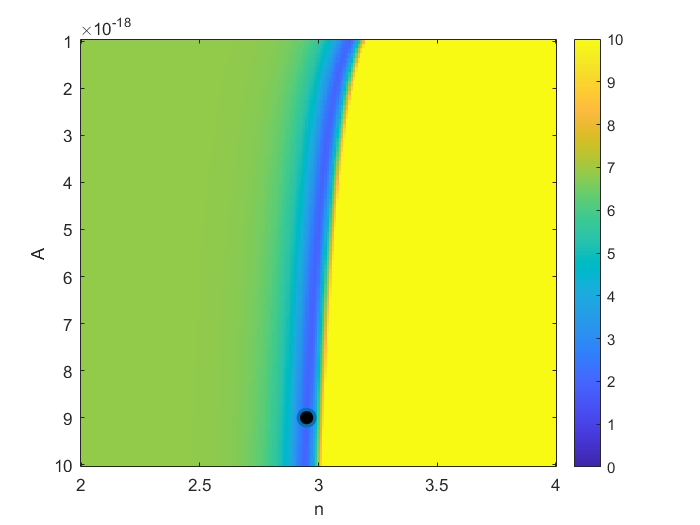
\includegraphics[width=0.8\columnwidth]{Q8.png} 
	\caption{The root mean square (RMS) error }
\end{figure}

The codes for ploting  root mean square (RMS) error (mean over all depths) as a function of A and n 

\begin{lstlisting}[language=Matlab,escapeinside=``]
figure(7);clf
imagesc(n,A,rms,[0 10]); colorbar
xlabel('n')
ylabel('A')
hold on
plot(n(y),A(x),'o','MarkerSize',10,'MarkerFaceColor','k','linewidth',2);
set(gca,'LineWidth',1,'FontSize',14,'FontWeight','bold')
print('Q8','-dpng')

\end{lstlisting}



\clearpage
\section*{Question 9 }

\begin{problem}
 Find the optimum values of A and n using the gradient search method with MATLAB's fminsearch function.
	
\end{problem}

\subsection*{Answer}

The result from the gradient search method is that optimum A=2.45179925070370e-15, n=2.49941300385653 and the regarding RMSE=1.85644257693787.

The codes for  finding the optimum values of A and n using the gradient search method
 
 \begin{lstlisting}[language=Matlab,escapeinside=``]
fh=@(An)physics(depth,vel,An) % function handle, A can be tuned to data in v,z
A0=[A(x) n(y)];%give the initial value
[Abest,fval] = fminsearch(fh,A0) %use fminsearch to find optimal A and n
\end{lstlisting}
 
The physics function used in above codes are defined by:

 \begin{lstlisting}[language=Matlab,escapeinside=``]
function [rms]=physics(depth,vel,An)
% INPUTS:  x= independent variabe
%          y = dependent variable
%          An = parameters [A,n]
g=9.8; % [m/s^2]
rho=917; % [kg/m^3]
theta=10*pi/180; % convert slope angle to rad
um3=vel(1)-An(1).*(rho*g*sin(theta)).^An(2).*depth.^(An(2)+1); % Eq 6 in HW3
rms=sqrt(mean((um3-vel).^2)); % RMSE for each combo of n and A
end
\end{lstlisting}

\clearpage
 
 \section*{Question 10 }
 
 \begin{problem}
Randomly sample 90\% of the dataset and find the optimum value of A using the gradient search method,
and repeat 1000 times. Plot the distribution of A and the RMS error (over all depths) in the model using a
relative density histogram.
 	
 \end{problem}
 
 \subsection*{Answer}
 Because this quesion only requires the find optimum values of A, I fix the n that find in last question. In this way, we can get a better result. 
 
 The relative density histogram
 \begin{figure}[htbp]
 	\centering
 	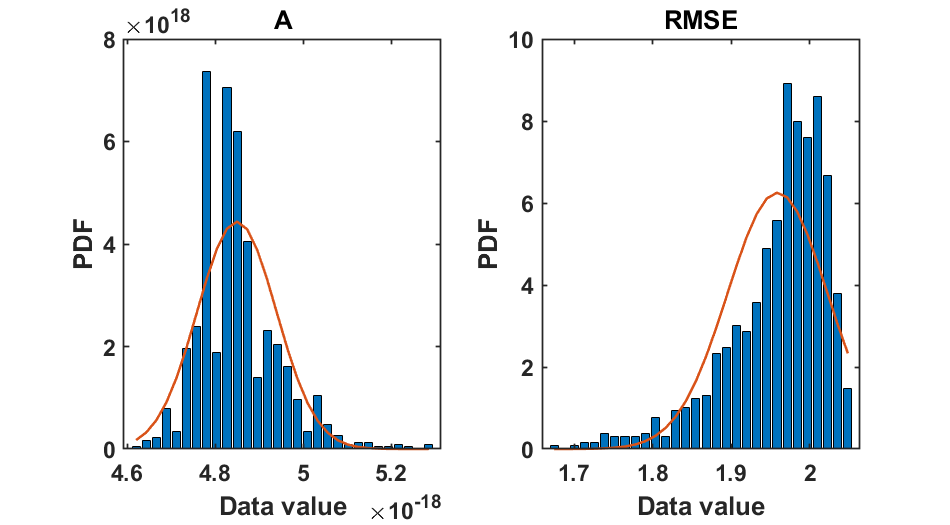
\includegraphics[width=1\columnwidth]{Q10.png} 
 	\caption{Plot the distribution of A and the RMS error }
 \end{figure}
 
The codes for randomly sampling 90\% of the dataset and find the optimum value of A using the gradient search method,
 
  \begin{lstlisting}[language=Matlab,escapeinside=``]

pTrain=0.9;%define the pecent that's used in polynomial fit
nMC=1000; %times for Monte-Carlo
rmseCV2=zeros(nMC,1); % initializing
u1=vel(1);

for p=1:nMC
[trainset, ~] = getTrainTest([depth vel],pTrain);%get 90% data
ztrain=trainset(:,1); % depths for training
vtrain=trainset(:,2); % velocity for training
fh=@(A)physics1(ztrain,vtrain,u1,A); % function handle, A can be tuned to data in v,z
A0=Abest(1);% initial guess of A
[Abest1,fval1] = fminsearch(fh,A0); %find the best parameters, and get the error
Aall(p)=Abest1;% store the A
rmseCV2(p)=fval1;% store the RMSE
end

bins=30;
figure
subplot(1,2,1)
plotRDH(Aall,bins);
title('A')
set(gca,'LineWidth',1,'FontSize',14,'FontWeight','bold')
subplot(1,2,2)
plotRDH(rmseCV2,bins);
title('RMSE')
set(gca,'LineWidth',1,'FontSize',14,'FontWeight','bold')
print('Q10','-dpng')

 \end{lstlisting}
 
 The physics1 function used in this problem.
  \begin{lstlisting}[language=Matlab,escapeinside=``]
 function [rms]=physics1(depth,vel,u1,A)
 % INPUTS:  x= independent variabe
 %          y = dependent variable
 %          An = parameters [A,n]
 g=9.8; % [m/s^2]
 rho=917; % [kg/m^3]
 n=3;% use a fixed n
 theta=10*pi/180; % convert slope angle to rad
 um3=u1-A.*(rho*g*sin(theta)).^n.*depth.^(n+1); % Eq 6 in HW3
 rms=sqrt(mean((um3-vel).^2)); % RMSE for each combo of n and A
 end
 \end{lstlisting}
 
 
\clearpage

 \section*{Question 11 }

\begin{problem}
Plot the mean optimum values of A and its standard deviation with vertical errorbars on your figure from \#7.	
\end{problem}

\subsection*{Answer}



The plot:
 \begin{figure}[htbp]
	\centering
	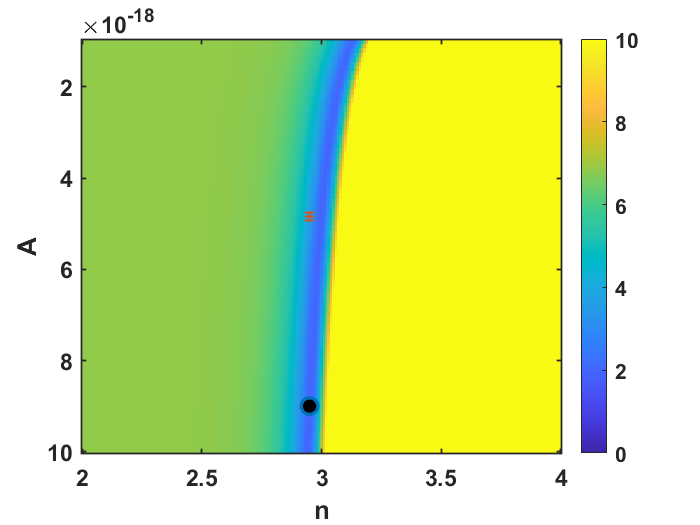
\includegraphics[width=1\columnwidth]{Q11.png} 
	\caption{Plot the distribution of A and the RMS error }
\end{figure}

The codes for ploting the mean optimum values of A and its standard deviation with vertical errorbars

  \begin{lstlisting}[language=Matlab,escapeinside=``]
figure(7)
hold on
%Plot the mean optimum values of A and its standard deviation with vertical errorbars
errorbar(n(y),mean(Aall),std(Aall),'+','linewidth',1)
set(gca,'LineWidth',1,'FontSize',14,'FontWeight','bold')
\end{lstlisting}

\clearpage

 \section*{Question 12 }

\begin{problem}
For each of A and model RMS error, use the normal distribution model to generate 1000 simulated values
with the mean and standard deviations from your Monte-Carlo simulations.	
\end{problem}

\subsection*{Answer}

The codes for generating 1000 simulated values
with the mean and standard deviations from the Monte-Carlo simulations
\begin{lstlisting}[language=Matlab,escapeinside=``]
A_sample=mean(Aall)+randn(1,1000)*std(Aall);%generate 1000 simulated values
%with the mean and standard deviations of the A from my Monte-Carlo simulations.

R_sample=mean(rmseCV2)+randn(1,1000)*std(rmseCV2);%generate 1000 simulated values
%with the mean and standard deviations of the RMSE from my Monte-Carlo simulations.
\end{lstlisting}

 \section*{Question 13 }

\begin{problem}
Use MATLAB's kstest2 function to compare the actual distributions from your Monte-carlo parameter
tting (\#9), with those simulated assuming a normal distribution (\#11).	
\end{problem}

\subsection*{Answer}

The codes for comparing the actual distributions from my Monte-carlo parameter
tting (\#9), with those simulated assuming a normal distribution (\#11).

\begin{lstlisting}[language=Matlab,escapeinside=``]
[h,p] = kstest2(Aall,A_sample) %compare the actual distributions of A with 
%simulated assuming a normal distribution

[h1,p1] = kstest2(rmseCV2,R_sample) %compare the actual distributions of RMSE with 
%simulated assuming a normal distribution
\end{lstlisting}

The output shows that h=1, p= 2.9934e-11; h1=1,p1=7.4350e-07. So the test rejects the null hypothesis the two samples(both A and RMSE versus regarding simulated samples) are from same distribution.

\end{document}
